\hline

\section{Jakub Pietraszko}


\newline


Problems with limits?
\[\lim_{x\to 8} \frac{1}{x-8} = \infty\]
Surprise your teacher using uncommon knowledge
\[ \lim_{x\to 5} \frac{1}{x-5} = \rotatebox{90}{5}\]
\emph{I will show out of the ordinary Lion on page \pageref{fig:Lion}}
\newline
\newline
Number ordered list
\begin{enumerate}
    \item Item 1
    \item Item 2
    \item Item 3
    \item ......
\end{enumerate}





Unordered list
\begin{itemize}
    \item Item 3
    \item Item 1
    \item Item 2
\end{itemize}



\begin{figure}[h]
\centering

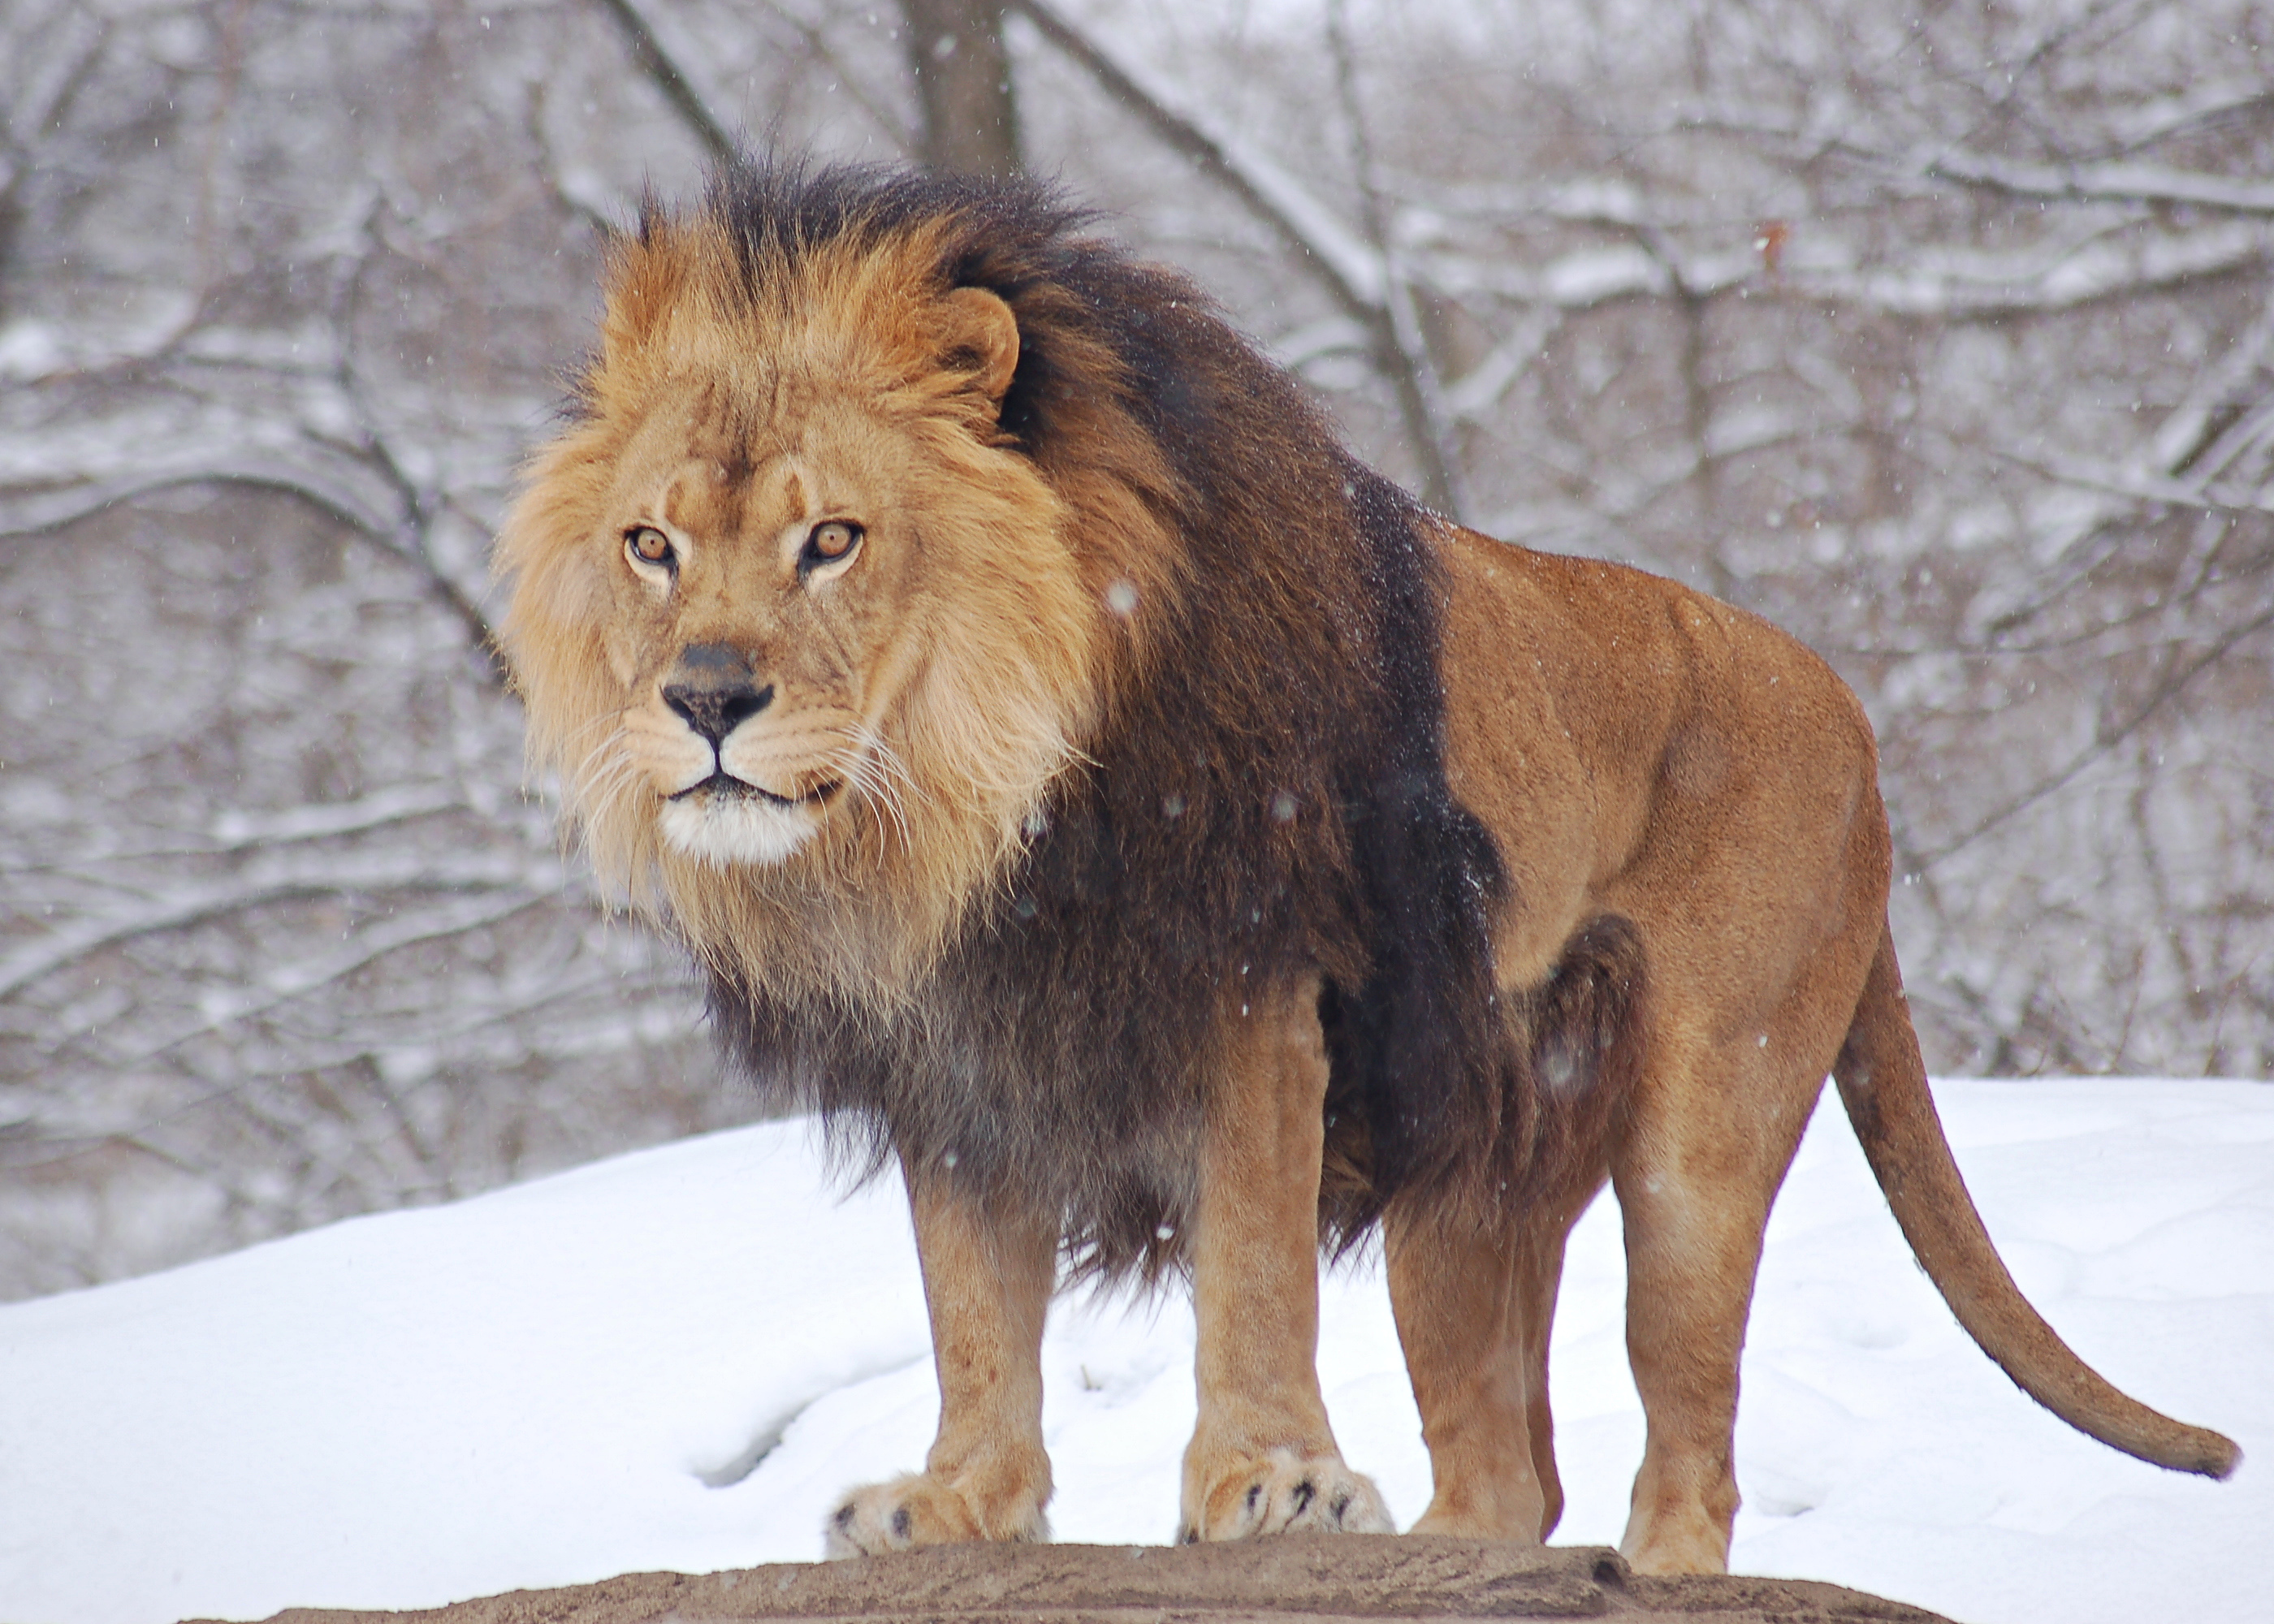
\includegraphics[width=0.7\textwidth]{pictures/Lew.jpg}

\caption{\label{fig:Lion}Lion}

\begin{flushleft}
The \textbf{lion} (\textbf{Panthera leo}) is a large cat of the genus Panthera native to \underline{Africa and India}. It has a muscular, broad-chested body, short, rounded head, round ears, and a hairy tuft at the end of its \emph{tail}.
\end{flushleft}

\newline

\begin{flushright}
\textit{Source Wikipedia}
\end{flushright}

\end{figure}


\begin{table}[h!]
\centering
\begin{tabular}{|l|lllll}
\hline
x & \multicolumn{1}{l|}{1} & \multicolumn{1}{l|}{2} & \multicolumn{1}{l|}{3} & \multicolumn{1}{l|}{4} & \multicolumn{1}{l|}{5} \\ \hline
1 & 1                      & 2                      & 3                      & 4                      & 5                      \\ \cline{1-1}
2 & 2                      & 4                      & 6                      & 8                      & 10                     \\ \cline{1-1}
3 & 3                      & 6                      & 9                      & 12                     & 15                     \\ \cline{1-1}
4 & 4                      & 8                      & 12                     & 16                     & 20                     \\ \cline{1-1}
5 & 5                      & 10                     & 15                     & 20                     & 25                     \\ \cline{1-1}
\end{tabular}


\caption{Simple Multiplications Table}


\end{table}


\newpage